\documentclass{standalone}

\usepackage{tikz}
\usepackage{pgfplots}

% You may be able to remove this if causing issues
\pgfplotsset{compat=1.11}

\begin{document}

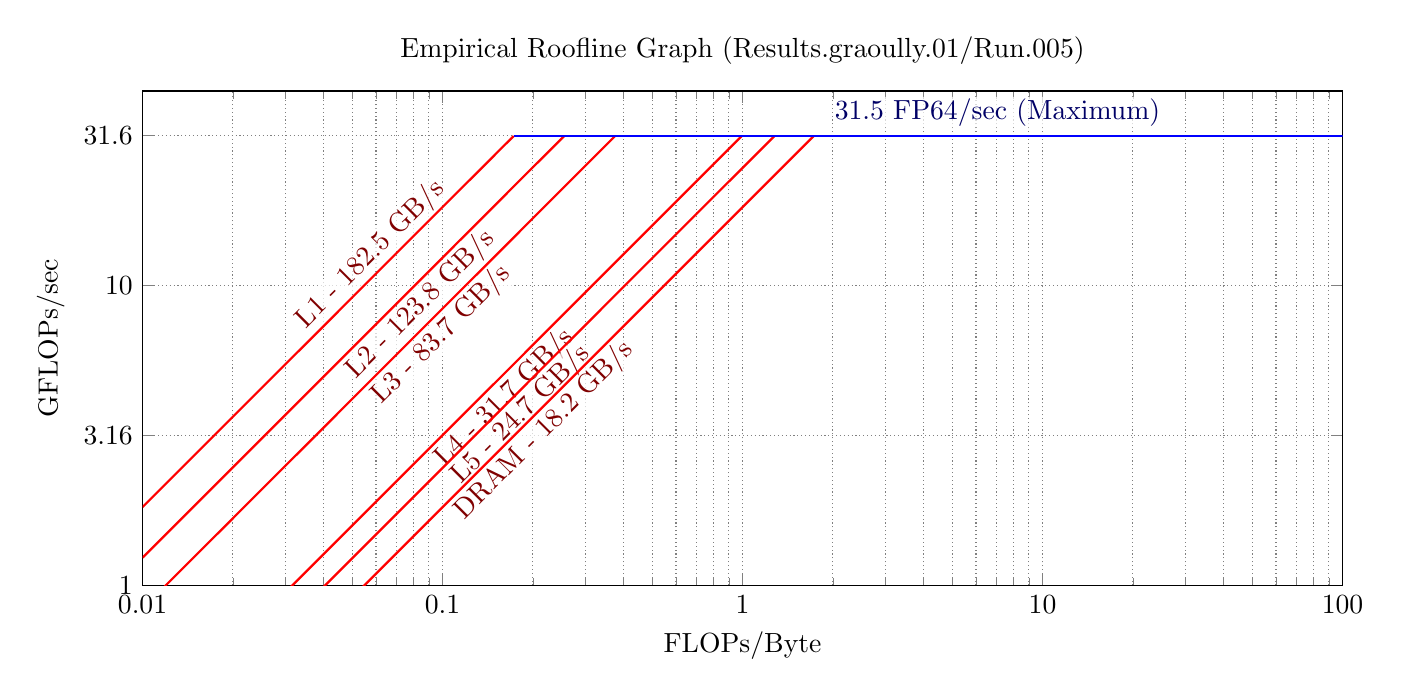
\begin{tikzpicture}
  \pgfplotsset {
    scale only axis,
    axis equal image,
    width=6in,
    /pgf/number format/1000 sep={},
    /tikz/maxline/.style={blue, thick, no marks},
    /tikz/memline/.style={red, thick, no marks},
    /tikz/maxlabel/.style={blue!40!black, right, fill=white, fill opacity=0.7, text opacity=1.0, rounded corners=2pt, inner sep=0.5pt},
    /tikz/memlabel/.style={red!50!black, rotate=45, right, fill=white, fill opacity=0.7, text opacity=1.0, rounded corners=2pt, inner sep=0.5pt}
  }

  \def\Xmin{1.000000e-02}
  \def\Xmax{1.000000e+02}

  \begin{loglogaxis}[
    title={Empirical Roofline Graph (Results.graoully.01/Run.005)},
    grid=both,
    grid style={black!50, densely dotted},
    xlabel= FLOPs/Byte,
    ylabel= GFLOPs/sec,
    xmin=\Xmin,
    xmax=\Xmax,
    ymin=1.000000e+00,
    ymax= ,
    log ticks with fixed point
    ]

    \node[maxlabel] at (axis cs: 2.0000000e+00,3.7824000e+01) {31.5 FP64/sec (Maximum)};
    \node[memlabel] at (axis cs: 3.3311452e-02,7.3551953e+00) {L1 - 182.5 GB/s};
    \node[memlabel] at (axis cs: 4.8929822e-02,5.0074214e+00) {L2 - 123.8 GB/s};
    \node[memlabel] at (axis cs: 5.9503982e-02,4.1175772e+00) {L3 - 83.7 GB/s};
    \node[memlabel] at (axis cs: 9.6737306e-02,2.5327586e+00) {L4 - 31.7 GB/s};
    \node[memlabel] at (axis cs: 1.0964530e-01,2.2345894e+00) {L5 - 24.7 GB/s};
    \node[memlabel] at (axis cs: 1.1240223e-01,1.6943940e+00) {DRAM - 18.2 GB/s};

    \addplot[memline, domain=(\Xmin:1.7273126e-01)] {1.8248000e+02*x};
    \addplot[memline, domain=(\Xmin:2.5454252e-01)] {1.2383000e+02*x};
    \addplot[memline, domain=(\Xmin:3.7644811e-01)] {8.3730000e+01*x};
    \addplot[memline, domain=(\Xmin:9.9494949e-01)] {3.1680000e+01*x};
    \addplot[memline, domain=(\Xmin:1.2781833e+00)] {2.4660000e+01*x};
    \addplot[memline, domain=(\Xmin:1.7280702e+00)] {1.8240000e+01*x};
    \addplot[maxline, domain=(1.7273126e-01:\Xmax)] {3.1520000e+01};

  \end{loglogaxis}
\end{tikzpicture}

\end{document}
